\documentclass[10pt,journal]{IEEEtran}\usepackage{longtable}
\usepackage{graphicx} 
\usepackage{sidecap}
\usepackage{balance}
\usepackage{amsmath}
%\usepackage{cite}
\usepackage{amssymb}
\usepackage{amssymb}
\newcommand*{\QEDA}{\hfill\ensuremath{\blacksquare}}%
\newcommand*{\QEDB}{\hfill\ensuremath{\square}}%
\usepackage{siunitx}
\usepackage[none]{hyphenat}
\usepackage[margin=0.7in]{geometry}
\usepackage{esvect}
\usepackage{braket}
\usepackage{listings}
\usepackage{epstopdf}
\usepackage{subfigure}
\usepackage{color} %red, green, blue, yellow, cyan, magenta, black, white
\usepackage{verbatim}
\usepackage{mwe}
\usepackage{array}
\newcolumntype{$}{>{\global\let\currentrowstyle\relax}}
\newcolumntype{^}{>{\currentrowstyle}}
\newcommand{\rowstyle}[1]{\gdef\currentrowstyle{#1}%
  #1\ignorespaces
}
\usepackage{hhline}
\definecolor{mygreen}{RGB}{28,172,0} % color values Red, Green, Blue
\definecolor{mylilas}{RGB}{170,55,241}
\graphicspath{{Figures/}}
\DeclareSIUnit\uvrms{\micro\volt{}_{RMS}}
\DeclareSIUnit\mvrms{\milli\volt{}_{RMS}}

\begin{document}
\lstset{language=Matlab,%
    %basicstyle=\color{red},
    breaklines=true,%
    morekeywords={matlab2tikz},
    keywordstyle=\color{blue},%
    morekeywords=[2]{1}, keywordstyle=[2]{\color{black}},
    identifierstyle=\color{black},%
    stringstyle=\color{mylilas},
    commentstyle=\color{mygreen},%
    showstringspaces=false,%without this there will be a symbol in the places where there is a space
    numbers=left,%
    numberstyle={\tiny \color{black}},% size of the numbers
    numbersep=9pt, % this defines how far the numbers are from the text
    emph=[1]{for,end,break},emphstyle=[1]\color{red}, %some words to emphasise
    %emph=[2]{word1,word2}, emphstyle=[2]{style},    
}




%%%%%%%%%%%%%%%%%%%%%%%%%%%%%%%%%%%%%%%%%%%%%%%%%%%%%%%%%%%%%%%%%%%%%%%%%%%%%%%%%%%%%%%%%%
\title{EE 315\\Final Project}
\author{Thomas Flores and Samuel Lenius}
\date{\today}
\maketitle
%%%%%%%%%%%%%%%%%%%%%%%%%%%%%%%%%%%%%%%%%%%%%%%%%%%%%%%%%%%%%%%%%%%%%%%%%%%%%%%%%%%%%%%%%%

%%%%%% ABSTRACT %%%%%%%
\begin{abstract}
\lipsum[1]
\end{abstract}
%%%%%%%%%%%%%%%%%%%%%


%%%%%%% INTRODUCTION %%%%%%%%%%
\section{Introduction}
\lipsum[1-3]
%%%%%%%%%%%%%%%%%%%%%%%%%%%%

%%%%%%% COMPARATOR DESIGN %%%%%%%%%%%%
\section{Comparator}
\begin{figure}[tb]
\begin{center}
\includegraphics[width=1\columnwidth]{StrongArmLatch.pdf}
\caption{Circuit topology for the strong arm latch comparator.}
\label{fig:StrongArmLatch}
\end{center}
\end{figure}
Proper optimization of the comparator element in the SAR ADC will provide the greatest improvement in our figure of merit, as it will ultimately set the maximum speed of our design. Given that our figure of merit is proportional to the power consumed for each decision, the ideal design includes a dynamic comparator which only draws current during the decision time. For this reason, we choose the Strong Arm Latch \cite{Razavi:bp} for its energy efficiency and simple design.

To size our comparator to first order, we begin by considering the required noise specification of the total SAR ADC. We can derive the maximum noise power for our full-scale signal power as
\begin{equation}
\sigma_{n,in}^2=\frac{P_{sig}}{10^{SNR_{spec}/10}}=\frac{\frac{\left(0.5V_{FS}\right)^2}{2}}{10^{\frac{SNR_{spec}}{10}}}
\end{equation}
Because we are designing to first order and expect some noise contribution from the other blocks, we impose a slightly higher noise spec of \SI{60}{\decibel}. This gives an input referred noise requirement of $\sigma_{n,in}=\SI{707.11}{\uvrms}$ for $V_{FS}=\SI{2}{\volt}$.

We approximate the input referred noise for the strong arm latch as
\begin{equation}
\sigma_{n,in}^2\approx\frac{8\gamma}{A_v}\frac{kT}{C_{P,Q}}
\label{eq:InputNoise}
\end{equation}
where the gain $A_v$ during the amplification phase can be approximated as
\begin{equation}
A_v\approx\frac{g_{m1,2}}{I_D}V_{tn}
\label{eq:StrongArmGain}
\end{equation}
We select $\frac{g_m}{I_D}=15$ as this provides a reasonable tradeoff between speed and power of the transistor (SHOW CURVE?). From simulations, we find that the approximate threshold voltage $V_{tn}\approx\SI{250}{\milli\volt}$ for our nmos devices. We can then solve for the minimum capacitance necessary nodes P and Q using Equations \ref{eq:InputNoise}, \ref{eq:StrongArmGain}, and $\sigma_{n,in}=\SI{707}{\uvrms}$ 
\begin{equation}
C_{P,Q}\geq\frac{8\gamma}{A_v}\frac{kT}{\sigma_{n,in}^2}\rightarrow C_{P,Q}\geq\SI{14.79}{\femto\farad}
\end{equation}
To begin our design, we create a unit comparator constructed from some reasonable design choices. To maximize speed in the cross coupled inverters, we assume that pmos elements M5,6 should be twice the width of the nmos elements M3,4. To size M3,4, we must limit the widths so they do not signficantly contribute to the mismatch at the input. For our design with $A_v\approx3.5$, this means that $W3,4\geq\frac{1}{3.5}W1,2$ due to the offset referral to the input. 

\begin{table}[h]
\caption{Widths for comparators. All lengths minimum length $L=\SI{90}{\nano\metre}$}
\begin{center}
\begin{tabular}{c|c|c|c}
\hline \rowstyle{\bfseries} Transistor & \rowstyle{\bfseries} Unit & \rowstyle{\bfseries} First Order Design & \rowstyle{\bfseries} Optimized \\ \hline
M1,2 & \SI{1}{\micro\metre} & ? & ? \\ \hline
M3,4 & $\alpha W_{M1,2}$ & ? & ? \\ \hline
M5,6 & $2W_{M3,4}$ & ? & ? \\ \hline
M7 & ? & ? & ? \\ \hline
S1,2 & ? & ? & ? \\ \hline
S3,4 & ? & ? & ? \\ \hline
\end{tabular}
\end{center}
\label{tbl:ComparatorDesign}
\end{table}

%%%%%%%%%%%%%%%%%%%%%%%%%%%%%%%%%%


%%%%%%% BOOTSTRAPPED SWITCH DESIGN %%%%%%%%%%%%
\section{Track and Hold}
\begin{figure}[tbph]
\begin{center}
\includegraphics[width=1\columnwidth]{BootstrappedSwitch.pdf}
\caption{Circuit topology for the bootstrapped switch for improved linearity.}
\label{fig:BootstrappedSwitch}
\end{center}
\end{figure}
\lipsum[1-4]
%%%%%%%%%%%%%%%%%%%%%%%%%%%%%%%%%%



%%%%%%% DAC DESIGN %%%%%%%%%%%%
\section{9 Bit Capacitive DAC}

\begin{figure}[tbph]
\begin{center}
\includegraphics[width=1\columnwidth]{dac_optimization.eps}
\caption{Optimization of settling time vs device unit width.}
\label{fig:DacOptimization}
\end{center}
\end{figure}

% TODO(sam) reference
Here we implement a 9 bit capacitive constant common mode top plate sampling DAC as in [2013 Tripathi].

Each bit of the DAC is binary weighted with a single dummy value in the
sequence 1, 1, 2, 4, 8, 16, 32, 64, 128.
For each bit there is both the top plate sampled capacitor and the corresponding inverter cell.

In order to have equal time constants between capacitors and inverter cells, equal scaling parameters are applied to each, hence the device widths of the cells follow the same sequence as the capacitors.

One complication of this approach is that the electrical effort to drive the inverters scales with this same sequence. 
Hence as the driver inverters scale up, the sequence of gate drive buffers must as well for optimal delay and power consumption.
This leads to each DAC inverter cell being designed individually for the expected range of electrical effort of that cell across optimization.

% TODO(sam) put a real circuit here
\begin{figure}[tbph]
\begin{center}
\includegraphics[width=1\columnwidth]{dac_optimization.eps}
\caption{DAC inverter unit cells.}
\label{fig:DACUnitInverterSch}
\end{center}
\end{figure}

% TODO(sam) reference
Our initial implementation of the inverter cell followed [2013 Tripathi] however we found that by using an inverter and a pair of N-channel devices we were able to achieve lower total delay and settling time. 

The specific issue with a standard inverter cell was that as the DAC switched it's MSB or MSB-1 bits, the dV/dT induced currents through the P-channel devices of the MSB-1 and MSB-2 cells caused a disturbance that reduced the gate overvoltage, hence increasing channel resistance and lengthening the duration of the glitch. 

By using a pair of N-channel devices we have applied a much higher gate overvoltage, and additionally the switching glitches now increase the gate overvoltage, improving the recovery time for glitches.
The use of two N channel devices here reduces the total gate capacitance to drive by a factor of two while reducing the output node parasitic capacitance, hence reducing DAC power overall.

Using a criterion of settling to within 1/2 LSB our optimized design has a delay of 370ps.
Accounting for the 1\% parasitic capacitance to ground on the top plate of the DAC capciators, our DAC reference voltage is 606mV in this design. 

%%%%%%%%%%%%%%%%%%%%%%%%%%%%%%%%%%



%%%%%%% LOGIC DESIGN %%%%%%%%%%%%
\section{Asynchronous Reset Logic}

\begin{figure}[tbph]
\begin{center}
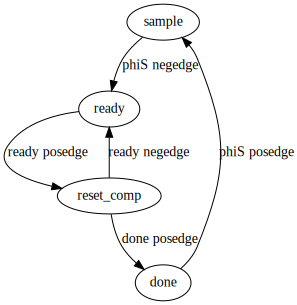
\includegraphics[width=1\columnwidth]{async.pdf}
\caption{State transition diagram for asynchronous reset logic.}
\label{fig:AsyncStateMachine}
\end{center}
\end{figure}

% TODO(sam) timing diagram

% TODO(sam) reference
In this ADC we implement asynchronous reset logic as in [2006 Chen]. The state machine that our asynchronous logic implements is as follows.

First the sampling clock edge rises, this opens the sampling gates and resets the internal state of the logic.

Second, the sampling clock drops and the asynchronous clock rises, enabling the dynamic comparator.

Third, the comparator makes a decision an one of it's two output lines drops. 
The outputs of the comparator are tied to the inputs of NAND gate as well as a buffer chain to drive the logic.
The reset state of the comparator has both lines high, hence the output of the NAND is low.
Once the comparator has made a decision, the output of the NAND is high, we call this signal 'Ready'. When Ready rises, we sample and shift one bit, and drop the asynchronous clock.

Fourth, after the bit is sampled, we reset the comparator. Here again we use the Ready signal to indicate that this step is finished. Once both of the comparator's output lines rise, the NAND's output will go to zero and we're prepared to convert the next bit. The Ready signal dropping will cause the clock to rise again, reenabling the comparator.

Fifth, once all 10 bits are shiftd out, we assert the done signal internally to the logic and the comparator is held in low power reset, ready for when the next sample comes in.

% TODO(sam) reference
[2006 Chen] gives us a speedup achievable for using asynchronous logic in equation 3 of that paper. Here Chen shows that as the number of bits in a converter increases that asynchronous processing will yield a speedup of up to a factor of two.
This means that for no additional energy per bit, that a converter using asynchronous logic can run twice as fast as it's synchronous counterpart. The decision to use asynchronous logic here is obvious.


%%%%%%%%%%%%%%%%%%%%%%%%%%%%%%%%%%


\bibliographystyle{IEEEtran}
\bibliography{IEEEabrv,References}
\end{document}


